\documentclass[11pt]{article} %article 文档
 \usepackage{color}
\usepackage{amsmath}
\usepackage{setspace}
\usepackage{graphicx}
\usepackage{caption}
\usepackage{hyperref}
\hypersetup{hidelinks,
	colorlinks=true,
	allcolors=black,
	pdfstartview=Fit,
	breaklinks=true}
\captionsetup[figure]{labelfont=bf, name=Figure, labelsep=period}
\newcommand{\reffig}[1]{Fig.\ref{#1}}
\setstretch{1.523} 
\title{COMP90007 Assignment 1}  %文章标题
\author{Student Name : Handan Yu\\ Student ID : 1235484}
\usepackage[a4paper,left=10mm,right=10mm,top=15mm,bottom=15mm]{geometry}  
\usepackage{enumerate}
\newtheorem{Q}{Ans}
\begin{document}
\date{}
\maketitle 
 \begin{Q}
 \end{Q}
\begin{enumerate}[Slot1.]
\item  in Group1 there are 5 stations(i.e., A, D, E, G, H) having data to transfer, which means there are collisions. So, DFS from the current node (assuming from the left 
node firstly), that is, moving to consider Group2.
\item  in Group2 there are  2 stations(i.e., A, D) having data to transfer, which also means there are collisions. So, move to consider Group4.
\item  in Group4 there is only a station(i.e., A) having data to transfer, and therefore station A competes successfully. Then BFS from the current node, that is, move to consider Group5.
\item  in Group5 there is only a station(i.e., D) waiting to transfer data, so that station D competes successfully. Then move to consider Group3.
\item  in Group3 there are 3 stations(i.e., E, G, H) having data to transfer, and then move on to its left node Group6 due to collisions.
\item  in Group6 there is a single station(i.e., E) having data to transfer, which means station E competes successfully. Then move to its peer node Group7.
\item  in Group7 there are still 2 stations(i.e., G, H) having data to transfer, so then G competes successfully at first and H right after.
\end{enumerate}
 \begin{Q}
 \end{Q}
(1)
 \begin{figure}[htbp]
 \centering
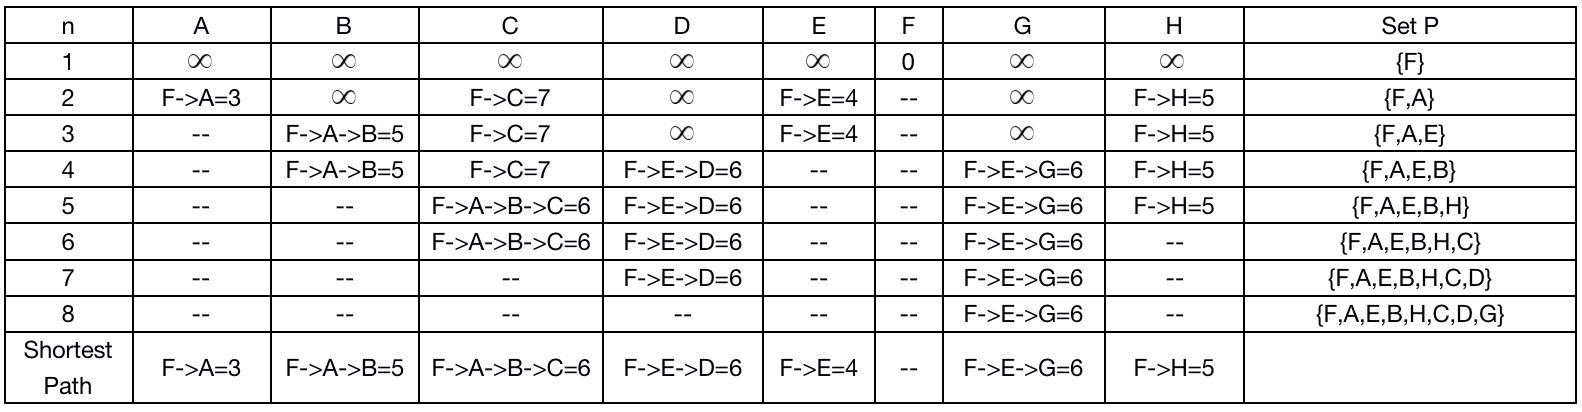
\includegraphics[height=4cm,width=15cm]{img/shortestpath1.png}
\caption{shortest paths from F to the other nodes }
 \end{figure}
 
 (2)
 If router E is offline, all of shortest path through E will be damaged. To be concrete, the shortest paths of D,G will be broken up. 
 
  \begin{figure}[htbp]
 \centering
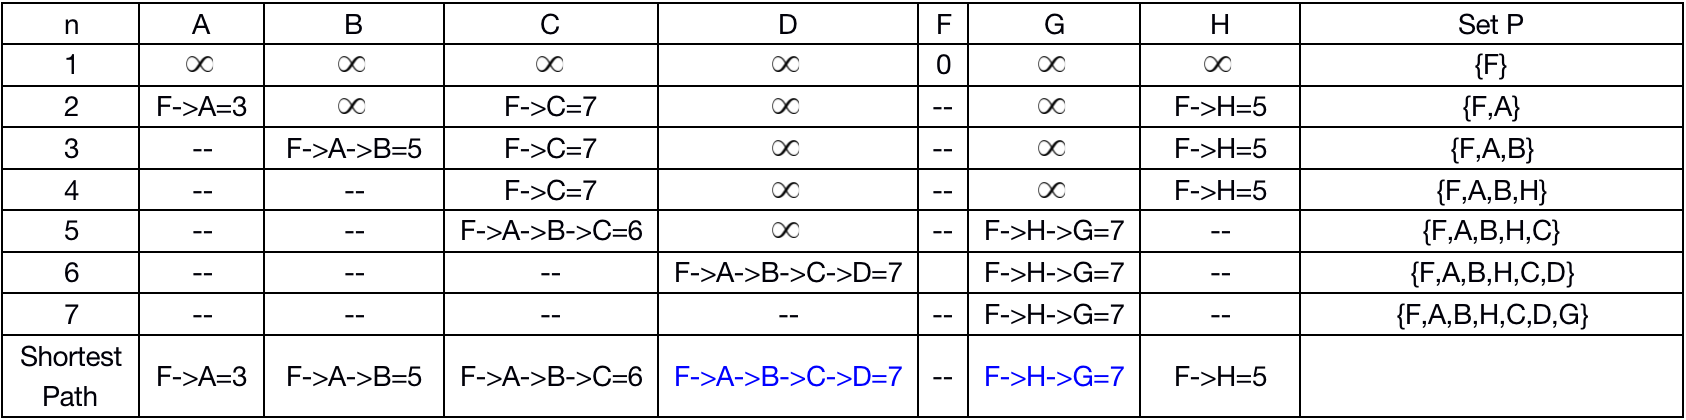
\includegraphics[height=4cm,width=15cm]{img/shortestpath2.png}
\caption{shortest paths from F to the other nodes (E error) }\label{shortestpath2}
 \end{figure}
 
 From \reffig{shortestpath2}, the shortest path from F to D will be F$\rightarrow$A$\rightarrow$B$\rightarrow$C$\rightarrow$D, which weight is 7. Also, the shortest path from F to G changes to F$\rightarrow$H$\rightarrow$G, which weight is 7.
 
 \begin{Q}
 \end{Q}
 
 (1)
 RPC is a function call in programming languages to send a message and get a reply back. UDP provides a protocol which allows the application can transmit encapsulated IP datagrams without a connection establishment, so that using UDP can eliminate overhead other than data communication and then help the RPC to communicate flexibly and  conveniently. Also, UDP is popular for local transport, confined to one LAN.  Furthermore, UDP provides an IP interface with multiplexing/demultiplexing capabilities and related transmission efficiencies, which can improve the performance of RPC. On the contrary, using TCP to send a message and get a reply will cause the additional overhead of setting up and tearing down a connection. 

(2) No matter during request or response, UDP gives RPC the freedom simply to ignore lost packets.

(3) When the RPC would be implemented under distribute system, or reliable, sequenced delivery is needed, a programmer might prefer to use TCP for RPC.

 \begin{Q}
 \end{Q}
 
 (1) 
 Bandwidth represents the rate of data transmission. If the bandwidth is too low, so that the speed of data transmission and download is less than the rate of video stream playback, and thus there will be frequent pauses and buffers in video playback, which will greatly affect the fluency of customers' viewing.
 
In terms of Jitter, Jitter is defined as the variation in packet arrival times. If there is a high jitter, a large cache must be used, which will directly cause greater delay and directly affect the quality of streaming media.

 (2)
Cache queuing. That is a buffer is established to store data for a long enough time so that the slowest packet can arrive in time before audio restore, so as to eliminate the adverse effect of delay,  
 
 (3)
 The cache queueing technique can also appropriate for a Videcoonferencing application. Since the data transmitted in a Videcoonferencing application is still video streaming. 
\begin{Q}
\end{Q}
 \begin{figure}[htbp]
 \centering
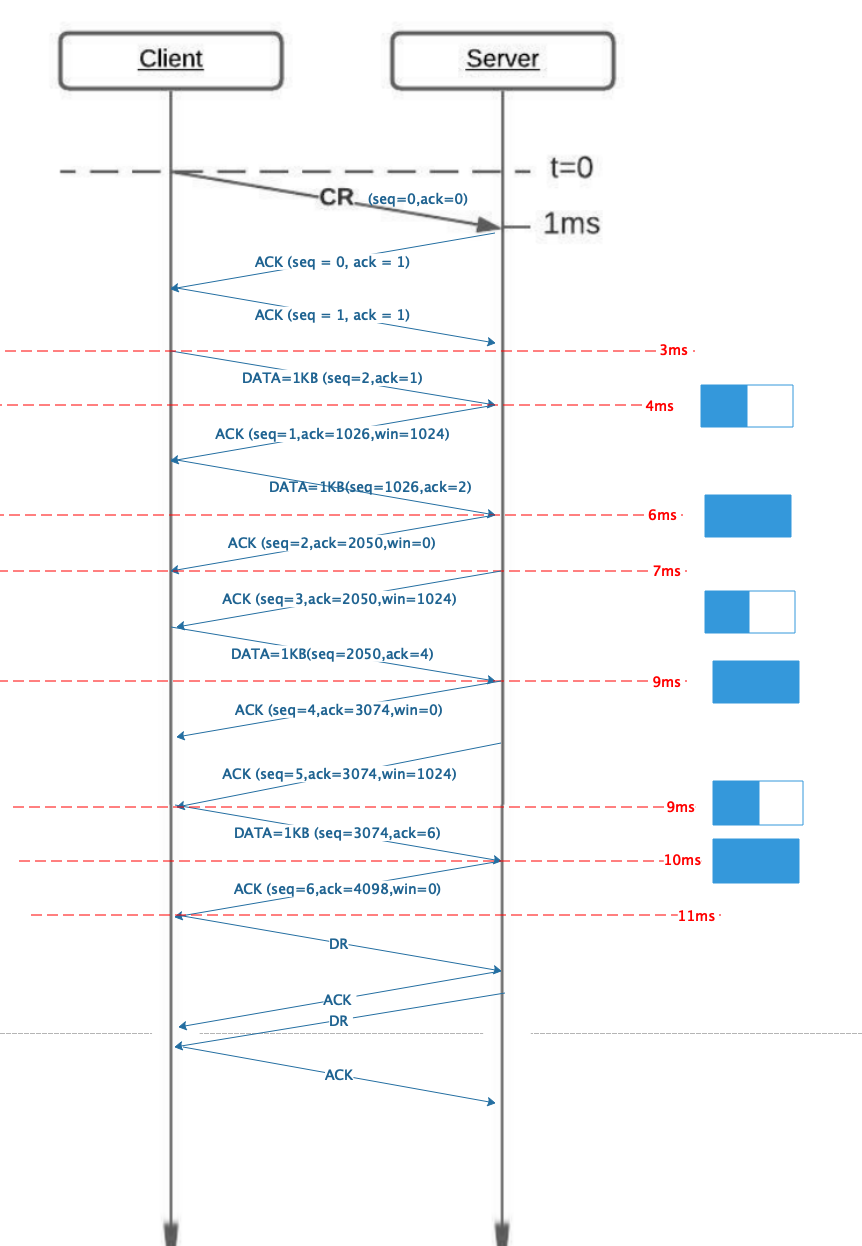
\includegraphics[height=13cm,width=10cm]{img/diagram.png}
\caption{sequence/timing diagram }
 \end{figure}

The first packet is trasmitted at 3ms and the last packet is received at 11ms. Therefore, the process take from commencing transmission of the first packet until 
the last packet is received takes 9ms.
\end{document}